\chapter{Analysis and Design of the MARVIS System}

The architecture of the proposed maritime surveillance system is designed as a multi-stage, modular pipeline in which each stage serves a specific purpose. Each module receives enhanced data from the previous stage and passes its output to the next stage, thereby improving process clarity and supporting real-time scalability. The system receives two types of input: a continuous video stream from a drone, \gls{cctv} camera, or satellite camera, and an \gls{ais} data stream containing vessel identifiers, positional coordinates, speed, and course data. These inputs are processed separately and then integrated in a sensor fusion layer that combines the spatial information from video-based tracking with the navigational information from \gls{ais} telemetry. The video pathway detects ships using \gls{yolov8}, preserves vessel identities using \gls{deepocsort}, and applies a homographic pixel-to-coordinate transformation to support geo-referencing. In parallel, the \gls{ais} pathway applies frame-rate interpolation and is then matched with the video pathway using the Haversine distance and Hungarian assignment algorithms. Enriched tracks, including \gls{mmsi}, speed, course, and ship type, are fused with noisy video detections using a Kalman filter. This filter reconciles the higher-frequency but less precise video stream with the sparser but more precise \gls{ais} observations to obtain a combined state estimate for the geographic position and velocity of each vessel. The resulting feature sequences, consisting of latitude, longitude, speed over ground, and trigonometric course encodings, are passed through an \gls{lstm} path predictor that estimates the future position of each vessel over the next K timesteps. Finally, a land-mask filter is applied as a post-processing stage to ensure that predicted paths remain within physically valid water areas.

\section{System Design Overview}

The proposed maritime surveillance system integrates multiple modules including \gls{ais} data acquisition, computer vision-based vessel detection, object tracking, trajectory prediction, collision analysis, and real-time visualization. Information obtained from maritime video streams and \gls{ais} data sources is processed to provide intelligent maritime surveillance and vessel monitoring.

The overall architecture of the proposed system is shown in Fig.~\ref{fig:architecture}.

\begin{figure}[H]
\centering
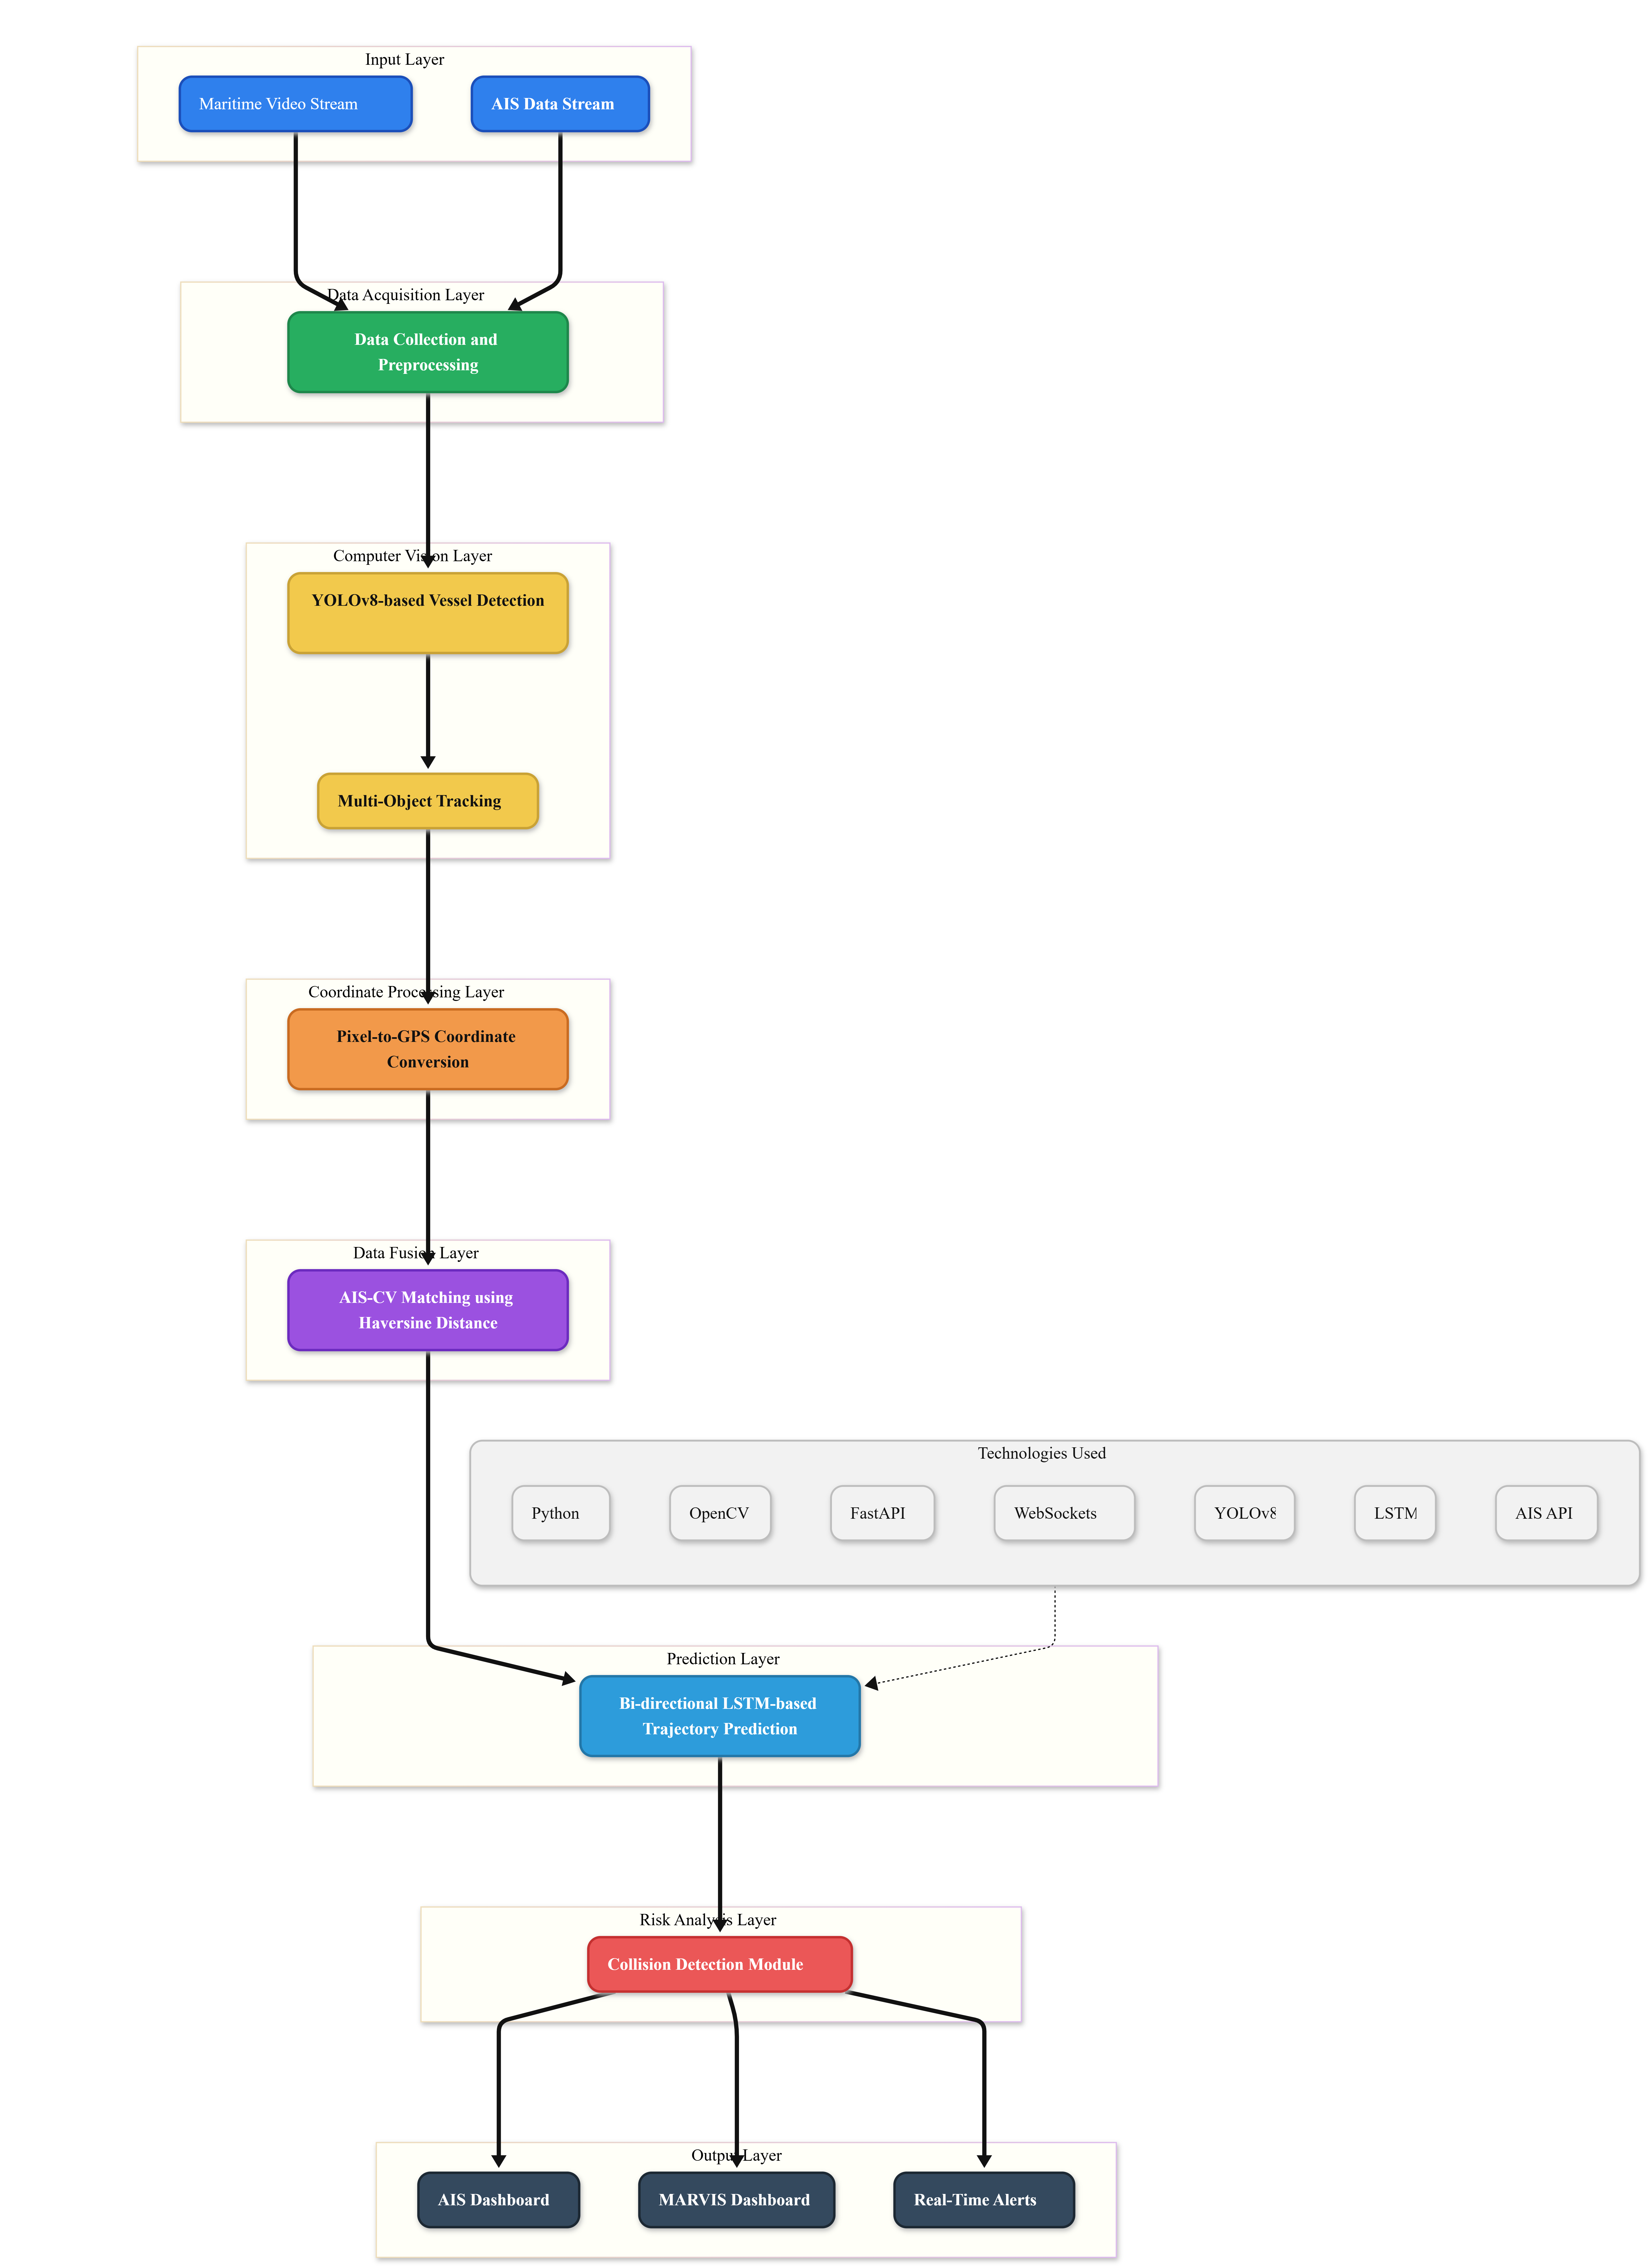
\includegraphics[width=0.95\textwidth]{Chapter3/Figures/system_architecture.png}
\caption{Overall Architecture of Proposed AI-Based Maritime Surveillance System}
\label{fig:architecture}
\end{figure}

\subsection{Specifications for the Design}
The proposed maritime surveillance system is designed to meet the following 
technical requirements. The system accepts continuous video input at a minimum 
resolution of 1280$\times$720 pixels and targets a processing throughput of up 
to 30 frames per second, ensuring real-time surveillance capability. The \gls{yolov8} 
detection module operates with a confidence threshold of 0.4 and an \gls{iou} threshold of 0.3 for \gls{nms}, balancing 
detection sensitivity against false-positive suppression. The \gls{deepocsort} tracker 
is configured with a maximum track age of 30 frames, a minimum confirmation hit 
count of 3, a detection threshold of 0.3, and cosine similarity as the distance 
metric for appearance-based \gls{reid} using the \gls{osnet} backbone.

The \gls{lstm} trajectory prediction module accepts a sequence of 50 timesteps as 
input and predicts the next 20 future positions per vessel. In the geospatial 
mapping module, pixel coordinates are transformed into geographic 
latitude--longitude pairs using a homographic transformation matrix computed via 
\texttt{cv2.findHomography} when ground-control calibration points are available, 
with a \gls{fov} linear approximation serving as the fallback. \gls{gps} positions 
derived from the pixel-to-coordinate transformation are further smoothed using a 
per-vessel Kalman filter with a constant-velocity motion model, which reduces the 
impact of detection jitter on downstream fusion and prediction. A land-mask 
post-processing stage validates all predicted vessel positions against a 
geographic water-area filter, ensuring that forecast trajectories remain within 
physically navigable regions. \gls{nvidia} \gls{cuda} acceleration is supported for real-time 
throughput. The system is implemented in Python using \gls{pytorch} as the deep learning 
framework and \gls{opencv} for video ingestion and frame-level processing.

A comprehensive pre-analysis was performed prior to the design of the system, 
involving dataset evaluation, model selection, and algorithmic benchmarking to 
ensure each component is well matched to the maritime surveillance environment.

\subsubsection{Use Case Analysis}

The use case diagram represents the interaction between users and the proposed maritime surveillance system. The major functionalities include video acquisition, vessel detection, tracking, trajectory prediction, and visualization. The diagram provides a high-level view of the system functionality and user interactions.
\begin{figure}[H]
\centering
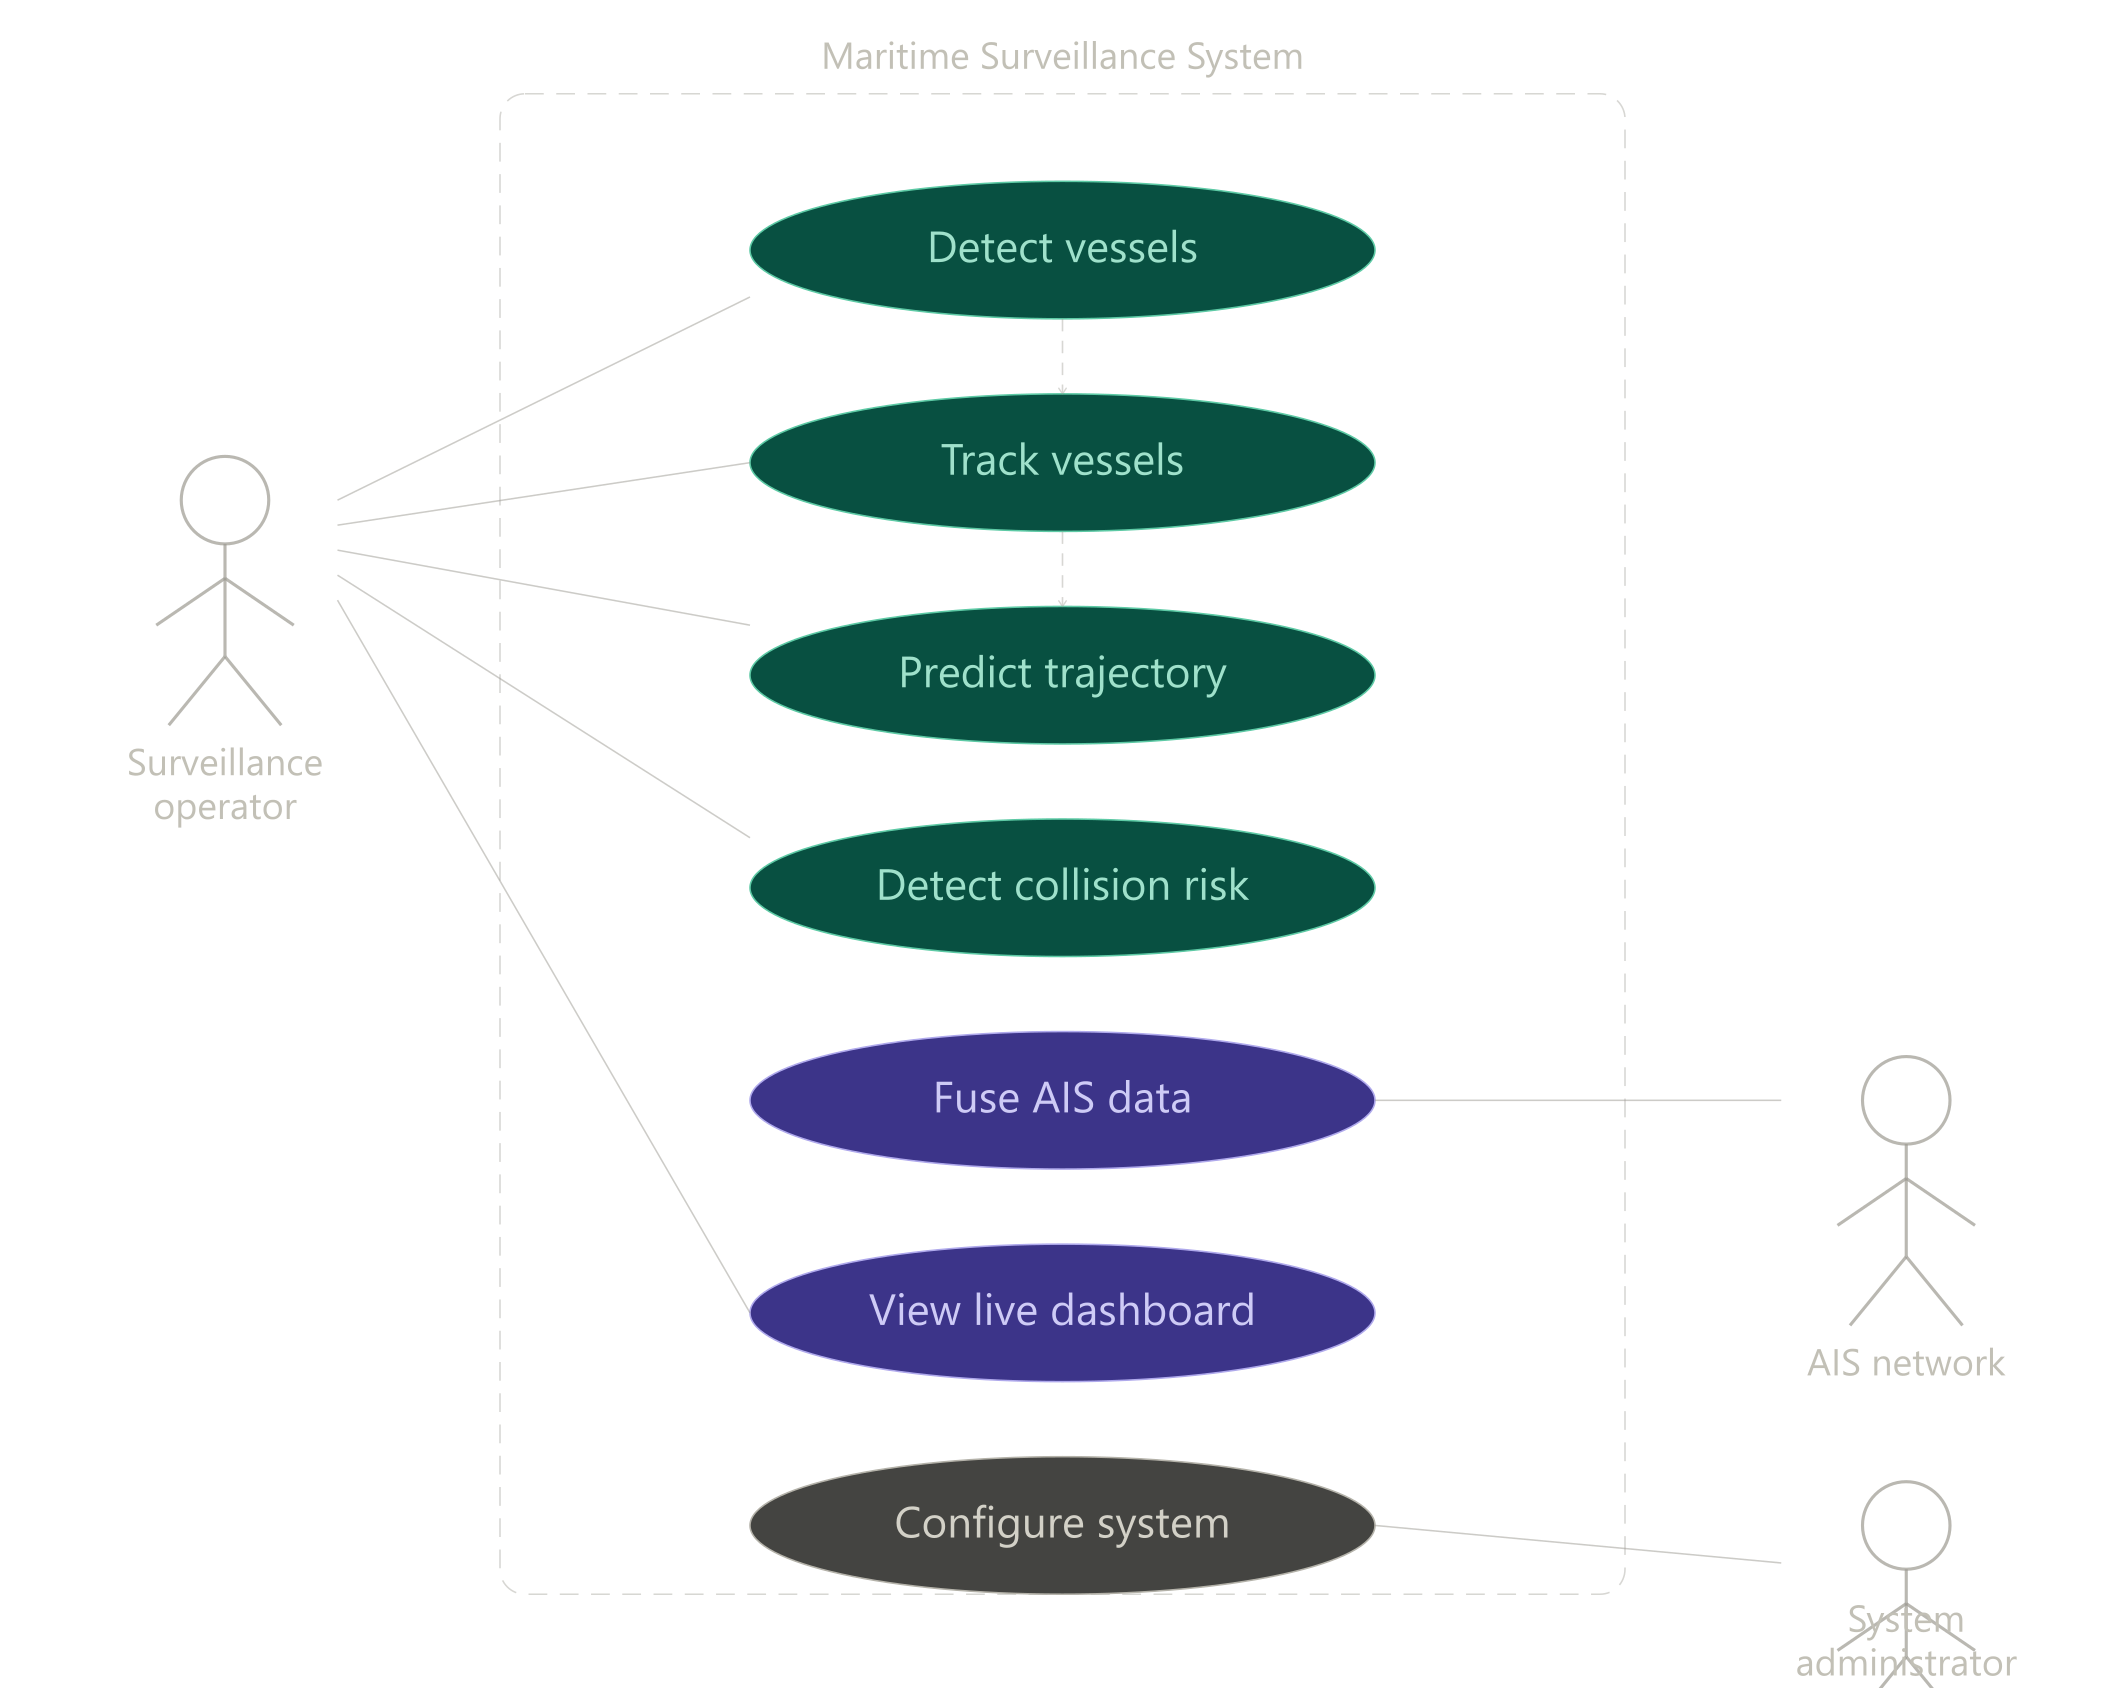
\includegraphics[width=0.95\textwidth]{Chapter3/Figures/fig3_use_case_diagram.png}
\caption{Use Case Diagram of the Maritime Surveillance System}
\label{fig:use_case}
\end{figure}

\subsection{Dataset Analysis}

The datasets used in this system serve two distinct purposes: the detection 
and fine-tuning of the \gls{yolov8} model, and the training of the \gls{lstm} trajectory 
prediction model. Each dataset was assessed for annotation quality, 
environmental diversity, vessel class distribution, and suitability for the 
maritime surveillance domain.

\subsubsection{Detection Dataset}

For vessel detection, the \textit{Kaggle Ships in Google Earth} dataset, 
accessed via the Roboflow platform (workspace: \texttt{robin-public}, project: 
\texttt{kaggle-ships-in-google-earth}, version 3), was used to fine-tune 
the \gls{yolov8} model. The dataset consists of aerial and satellite imagery of 
vessels annotated in \gls{yolo} format, with bounding boxes labelled for each vessel 
instance. Images were pre-processed and split into training, validation, and 
test partitions by the Roboflow pipeline. The dataset was selected for its 
diversity of sea states, illumination conditions, vessel scales, and occlusion 
scenarios, which are critical factors for a detection model intended to operate 
across varied real-world maritime surveillance conditions. Fine-tuning was 
performed on YOLOv8l for 70 epochs at an input resolution of 640$\times$640 
pixels using the dataset configuration file exported by Roboflow.

\subsubsection{Trajectory Prediction Dataset}

The \gls{smd} was used to train the \gls{lstm} trajectory 
prediction model. \gls{smd} is a publicly available benchmark captured using 
drone-mounted cameras over the Singapore Strait, one of the world's busiest 
maritime waterways, and provides ground-truth vessel trajectory annotations in 
the form of \texttt{TrackGT*.mat} files. Each \texttt{.mat} file contains a 
\texttt{Track} structure with per-vessel bounding boxes (\texttt{BB}) and a 
binary motion mask (\texttt{Motion}) indicating the frames in which each 
vessel is present. Trajectory centroids are extracted by computing the 
midpoint of each active bounding box:
\begin{equation}
    x_c = \frac{x_1 + x_2}{2}, \quad y_c = \frac{y_1 + y_2}{2}
    \label{eq:gps_conversion}
\end{equation}
Only trajectories with a minimum length of 50 frames are retained, ensuring 
that each sample contains sufficient history for the \gls{lstm} input window.

\subsubsection{Dataset Preprocessing}

The raw centroid sequences are processed by the \texttt{TrajectoryDataset} 
class using a sliding window of stride 1. Each window consists of 50 
consecutive timesteps as the input history and 20 subsequent timesteps as the 
prediction target. Positional coordinates are normalised by the video frame 
dimensions prior to feature construction:
\begin{equation}
    \hat{x} = \frac{x}{1920}, \quad \hat{y} = \frac{y}{1080}
    \label{eq:lat_offset}
\end{equation}
Per-frame velocity components are computed as first-order differences of the 
normalised positions:
\begin{equation}
    v_x^{(t)} = \hat{x}^{(t)} - \hat{x}^{(t-1)}, \quad 
    v_y^{(t)} = \hat{y}^{(t)} - \hat{y}^{(t-1)}
    \label{eq:haversine}
\end{equation}
The final input feature vector at each timestep is therefore 
$\mathbf{f}^{(t)} = [\hat{x}^{(t)},\; \hat{y}^{(t)},\; v_x^{(t)},\; 
v_y^{(t)}] \in \mathbb{R}^4$, giving an input tensor of shape 
$50 \times 4$ per sample. The processed dataset is split into training and 
validation sets in an 80:20 ratio using a fixed random seed of 42 for 
reproducibility. Training samples are loaded in shuffled mini-batches of 
size 32, while the validation set is evaluated in sequential order.

\subsubsection{Evaluation Protocol}

Model performance on the trajectory prediction task is quantified using two 
standard metrics. The \textit{Average Displacement Error} (\gls{ade}) measures the 
mean Euclidean distance between predicted and ground-truth positions across 
all predicted timesteps:
\begin{equation}
    \text{ADE} = \frac{1}{K} \sum_{k=1}^{K} 
    \sqrt{(\hat{x}_k - x_k)^2 + (\hat{y}_k - y_k)^2}
    \label{eq:LSTM1}
\end{equation}
The \textit{Final Displacement Error} (\gls{fde}) measures the Euclidean distance 
at the last predicted timestep only:
\begin{equation}
    \text{FDE} = \sqrt{(\hat{x}_K - x_K)^2 + (\hat{y}_K - y_K)^2}
    \label{eq:LSTM2}
\end{equation}
These metrics are computed separately for the \gls{lstm} model and for a kinematic 
linear baseline, and the percentage improvement of \gls{lstm} over the baseline is 
reported for both \gls{ade} and \gls{fde}.

\subsection{Detection Model Selection}

\gls{yolov8} was selected as the vessel detection backbone following a comparative 
evaluation of \gls{yolo}-family architectures including \gls{yolo}v5, \gls{yolo}v7, and 
\gls{yolo}v7-Tiny. The key differentiating factors in favour of \gls{yolov8} are its 
anchor-free detection head, its redesigned C2f backbone module, and its 
decoupled classification and regression branches. Anchor-free designs eliminate 
the need to predefine anchor box aspect ratios, which is particularly beneficial 
in maritime scenes where vessel aspect ratios vary significantly with viewing 
angle, distance, and vessel type. The optimised feature pyramid network in 
\gls{yolov8} improves multi-scale feature aggregation, enabling the model to detect 
both large cargo vessels occupying a large portion of the frame and small 
distant vessels spanning only a few pixels. This small-object detection 
capability is critical for the intended surveillance scenario, where vessels 
at range may occupy as few as 10$\times$10 pixels in a 1280$\times$720 frame. 
The Ultralytics \gls{yolov8} implementation additionally provides a unified Python 
\gls{api} compatible with \gls{pytorch}, facilitating integration with the downstream 
tracking and prediction pipeline. The YOLOv8n variant is used at runtime for 
detection speed, while the YOLOv8l variant was used during fine-tuning on 
the Roboflow maritime dataset.

\subsection{Tracking Algorithm Selection}

\gls{deepocsort} was selected as the multi-object tracking algorithm following 
evaluation against motion-only trackers. The fundamental limitation of 
motion-only trackers such as \gls{sort} is that identity assignment relies 
exclusively on bounding-box \gls{iou} overlap between consecutive frames. In dense 
maritime scenes where vessels travel in close proximity, cross paths, or are 
temporarily occluded by structures such as port infrastructure or other 
vessels, \gls{iou}-based matching produces frequent identity switches. \gls{deepocsort} 
addresses this by augmenting the cost matrix with an appearance similarity 
term derived from an \gls{osnet} \gls{reid} model, which embeds the visual 
appearance of each detected vessel into a descriptor vector. The combined 
cost matrix incorporates both spatial proximity and appearance consistency, 
reducing identity switches in occluded and crossing scenarios. Additionally, 
\gls{deepocsort} employs a Kalman filter per track to predict the expected bounding 
box position at the next frame, providing a robust motion prior when 
detections are temporarily absent. Tracks are confirmed after a minimum of 
3 consecutive detections and are retained for up to 30 frames without a 
matching detection before being discarded, preventing the proliferation of 
spurious track identities from transient false positives.

\subsection{Prediction Model Selection}

\gls{lstm} networks were selected for trajectory prediction in preference to Kalman 
filters and \gls{gru} variants. Kalman filters, while computationally efficient, 
operate under a linear constant-velocity motion assumption and cannot model 
the non-linear manoeuvring behaviour exhibited by maritime vessels, including 
course corrections, lane merging in traffic separation schemes, and 
speed-dependent turning arcs. \gls{gru} variants were considered as a lighter 
alternative to \gls{lstm} but were not selected because the additional gating 
complexity of \gls{lstm} — specifically the separate input, forget, and output gates 
— provides better retention of long-range temporal dependencies, which is 
necessary when a vessel's future heading is influenced by a turning manoeuvre 
that began many frames prior. The selected architecture is a \gls{seqtwo} \gls{lstm} with 
a bidirectional encoder and a soft attention mechanism, which allows the decoder 
to focus selectively on the most predictive frames in the input history rather 
than compressing the entire 50-timestep sequence into a single fixed vector. 
For vessels whose track history has not yet reached the 50-timestep threshold 
required by the \gls{lstm} input window, a kinematic fallback using linear regression 
over the available history is employed, ensuring that the system produces a 
trajectory estimate at every frame regardless of track length.

\subsubsection{Processing Pipeline Overview}

The proposed maritime surveillance system follows a structured processing pipeline that integrates maritime video streams with \gls{ais} telemetry information for intelligent vessel monitoring and prediction. Initially, video streams undergo vessel detection and object tracking, while \gls{ais} information is simultaneously processed and interpolated to improve temporal consistency. Subsequently, geographic coordinate transformation and sensor fusion mechanisms are applied to associate visual observations with \gls{ais} information.

The fused data are then processed through a filtering and feature extraction stage before being supplied to the trajectory prediction module. A \gls{bilstm} network analyses temporal movement patterns and predicts future vessel positions. The predicted outputs are further refined through land-mask constraints and subsequently utilized for visualization and collision analysis. The complete processing workflow of the proposed system is illustrated in Fig.~\ref{fig:pipeline}.

\begin{figure}[H]
\centering
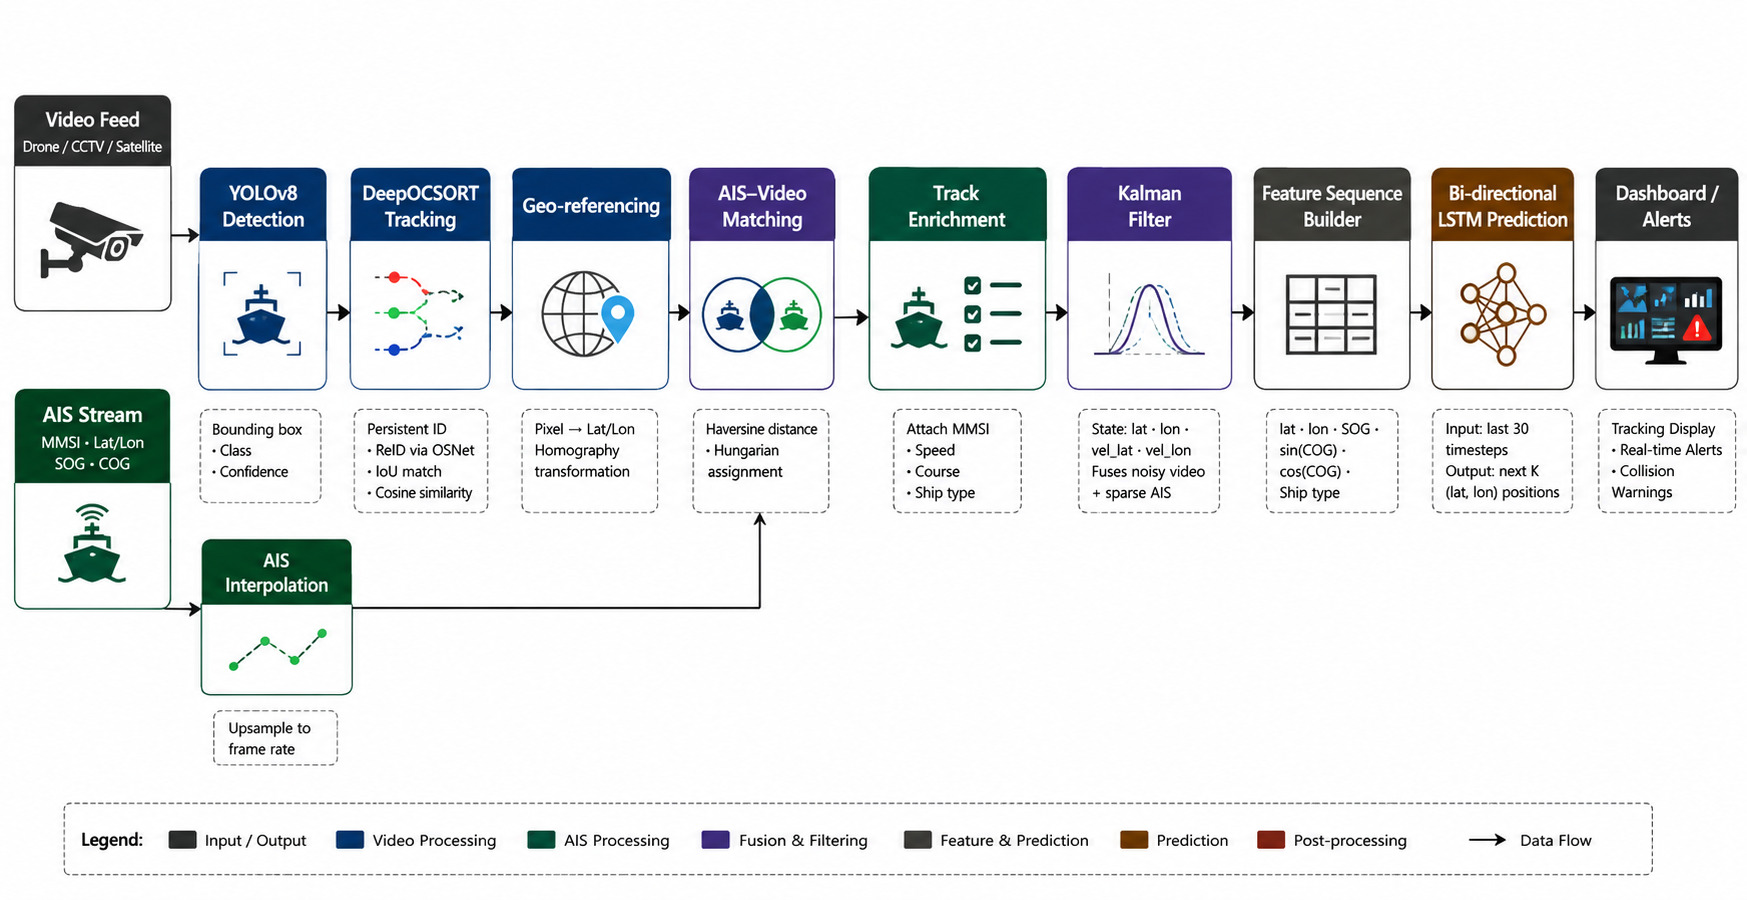
\includegraphics[width=0.85\textwidth]{Chapter3/Figures/process_pipeline.jpeg}
\caption{End-to-End Processing Pipeline of Proposed Maritime Surveillance System}
\label{fig:pipeline}
\end{figure}

\subsection{Sensor Fusion Strategy}

The complementary characteristics of video-based tracking and \gls{ais} telemetry 
present a natural opportunity for sensor fusion. Video-based tracking operates 
at frame rate, providing high-frequency positional updates, but the derived 
\gls{gps} coordinates are subject to noise introduced by pixel-to-coordinate 
projection errors and detection jitter. \gls{ais} telemetry, conversely, provides 
sparse updates at intervals of several seconds but carries precise \gls{gps} 
measurements alongside rich navigational metadata including \gls{mmsi}, vessel name, 
speed over ground (\gls{sog}), and \gls{cog}.

The fusion strategy adopted in this system is a nearest-neighbour association 
using the Haversine great-circle distance. For each camera-detected vessel 
whose pixel position has been converted to a \gls{gps} coordinate, the system queries 
the live \gls{ais} registry and computes the Haversine distance to every active \gls{ais} 
record. If the closest \gls{ais} vessel lies within the matching radius of 5.5\,km, 
the camera track is enriched with the \gls{ais} metadata: the \gls{mmsi}, vessel name, \gls{sog}, 
and \gls{cog} fields are copied into the camera detection record. Camera-detected 
vessels for which no \gls{ais} record exists within the search radius are classified 
as \textit{dark vessels} — non-cooperative targets that have either disabled 
their \gls{ais} transponder or are operating craft not required to carry \gls{ais} 
equipment. To reduce the effect of detection jitter on matching accuracy, \gls{gps} 
coordinates derived from pixel positions are smoothed using a per-vessel 
constant-velocity Kalman filter before the association step is performed.

\section{Data Flow Analysis}

The proposed maritime surveillance system processes information obtained from multiple sources and transforms it through different computational stages. Data flow analysis helps in understanding how information is exchanged between external entities, internal processing modules, and output interfaces within the system.

The system receives maritime video streams and \gls{ais} telemetry information as input. The acquired information undergoes vessel detection, tracking, coordinate transformation, data fusion, trajectory prediction, and visualization stages before generating outputs for surveillance and decision support.

\subsection{Level-0 Context Diagram}

The Level-0 Context Diagram provides a high-level representation of the interaction between external entities and the maritime surveillance system. The diagram illustrates how users, \gls{ais} data providers, and maritime video sources exchange information with the proposed system.


\begin{figure}[!htbp]
\centering
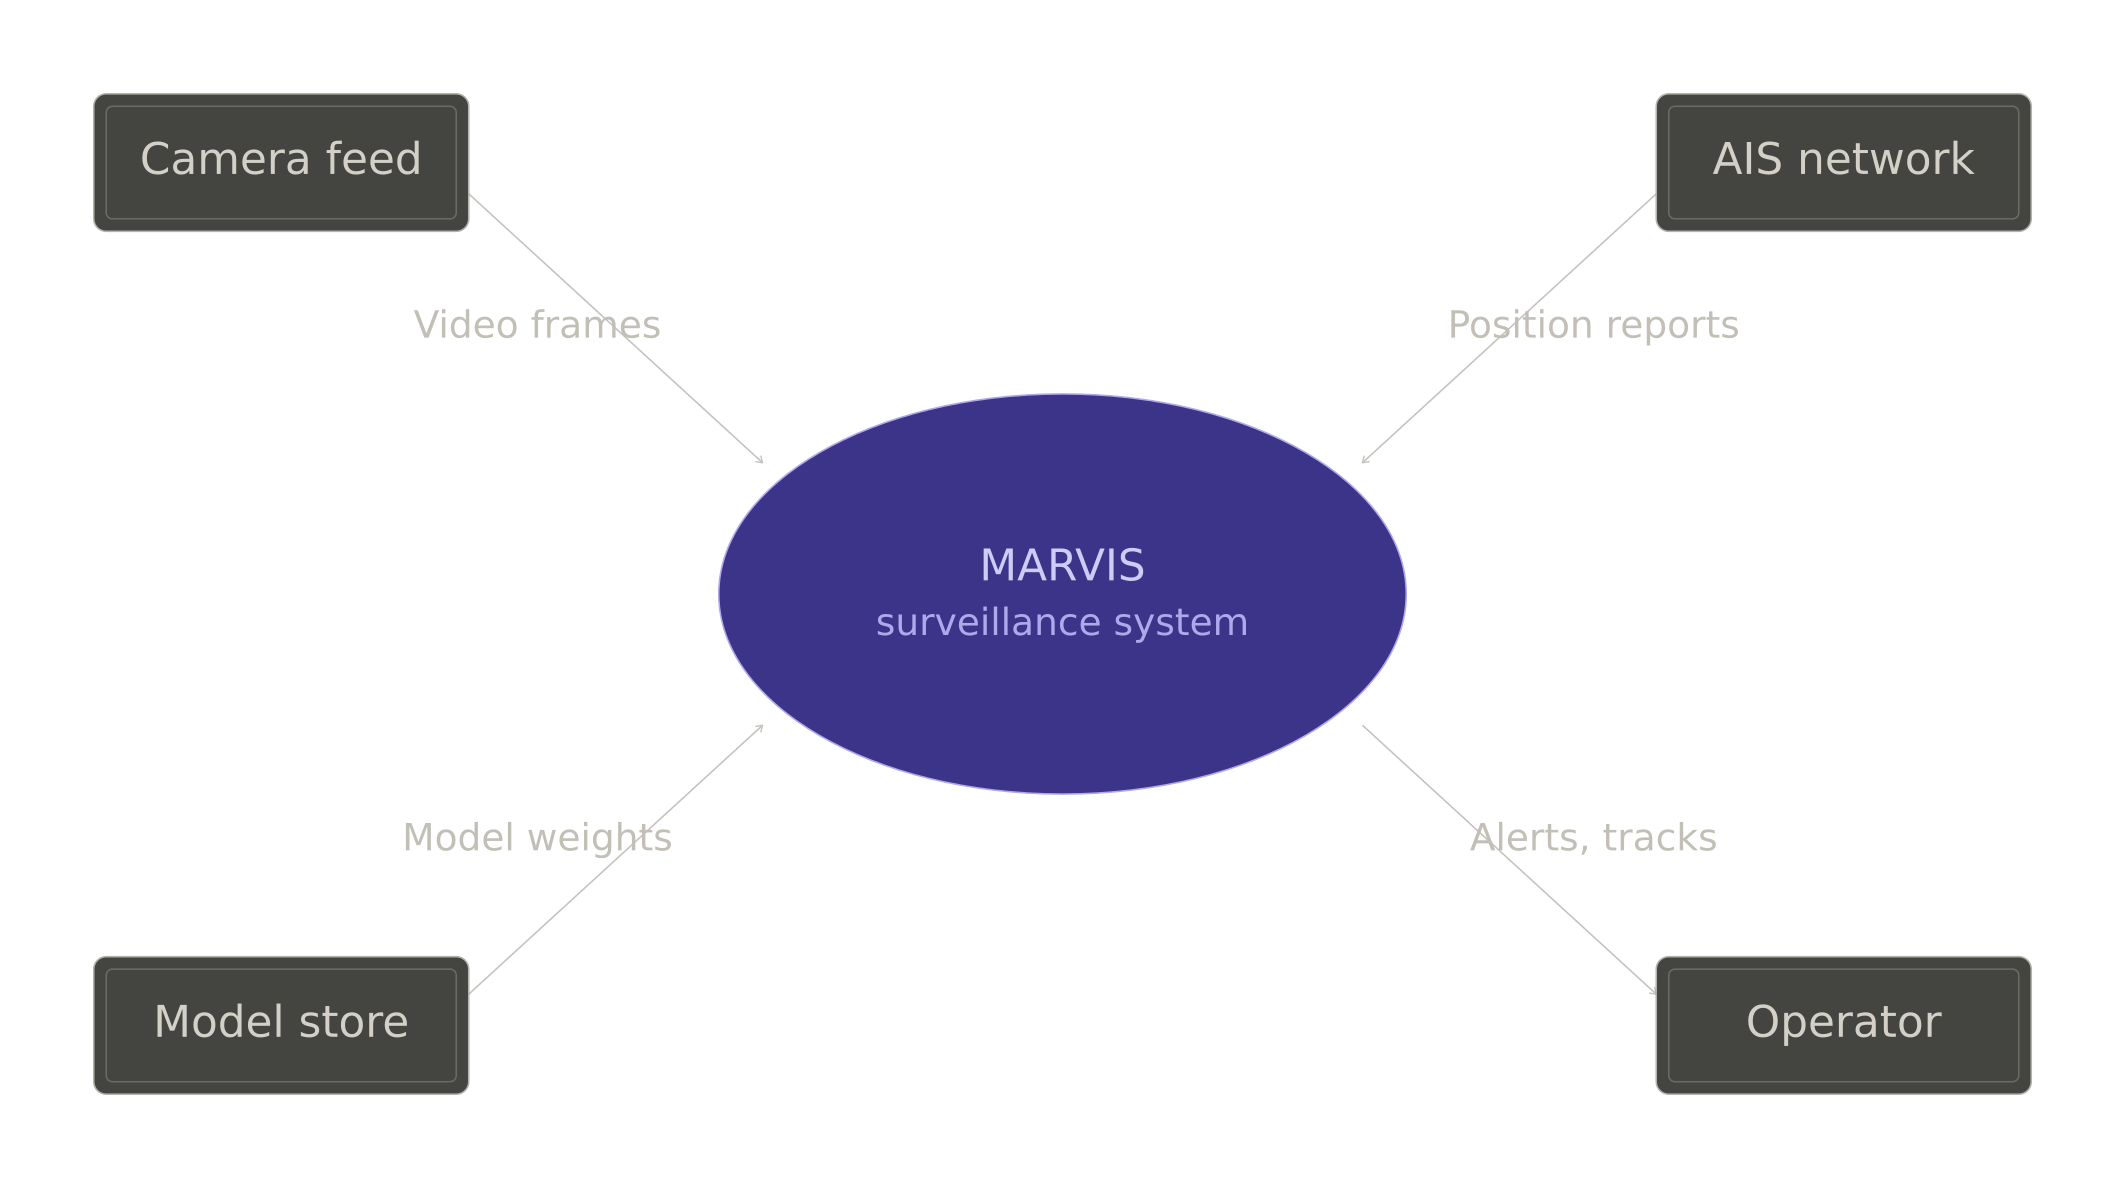
\includegraphics[width=0.95\textwidth]{Chapter3/Figures/dfd_level0_context.png}
\caption{Level-0 Context Diagram of Proposed Maritime Surveillance System}
\label{fig:dfd0}
\end{figure}

\subsection{Level-1 Data Flow Diagram}

The Level-1 Data Flow Diagram expands the internal operations of the proposed system and illustrates the flow of information across different processing modules. The workflow includes vessel detection, object tracking, coordinate transformation, \gls{ais} fusion, trajectory prediction, collision analysis, and dashboard visualization.

\begin{figure}[!htbp]
\centering
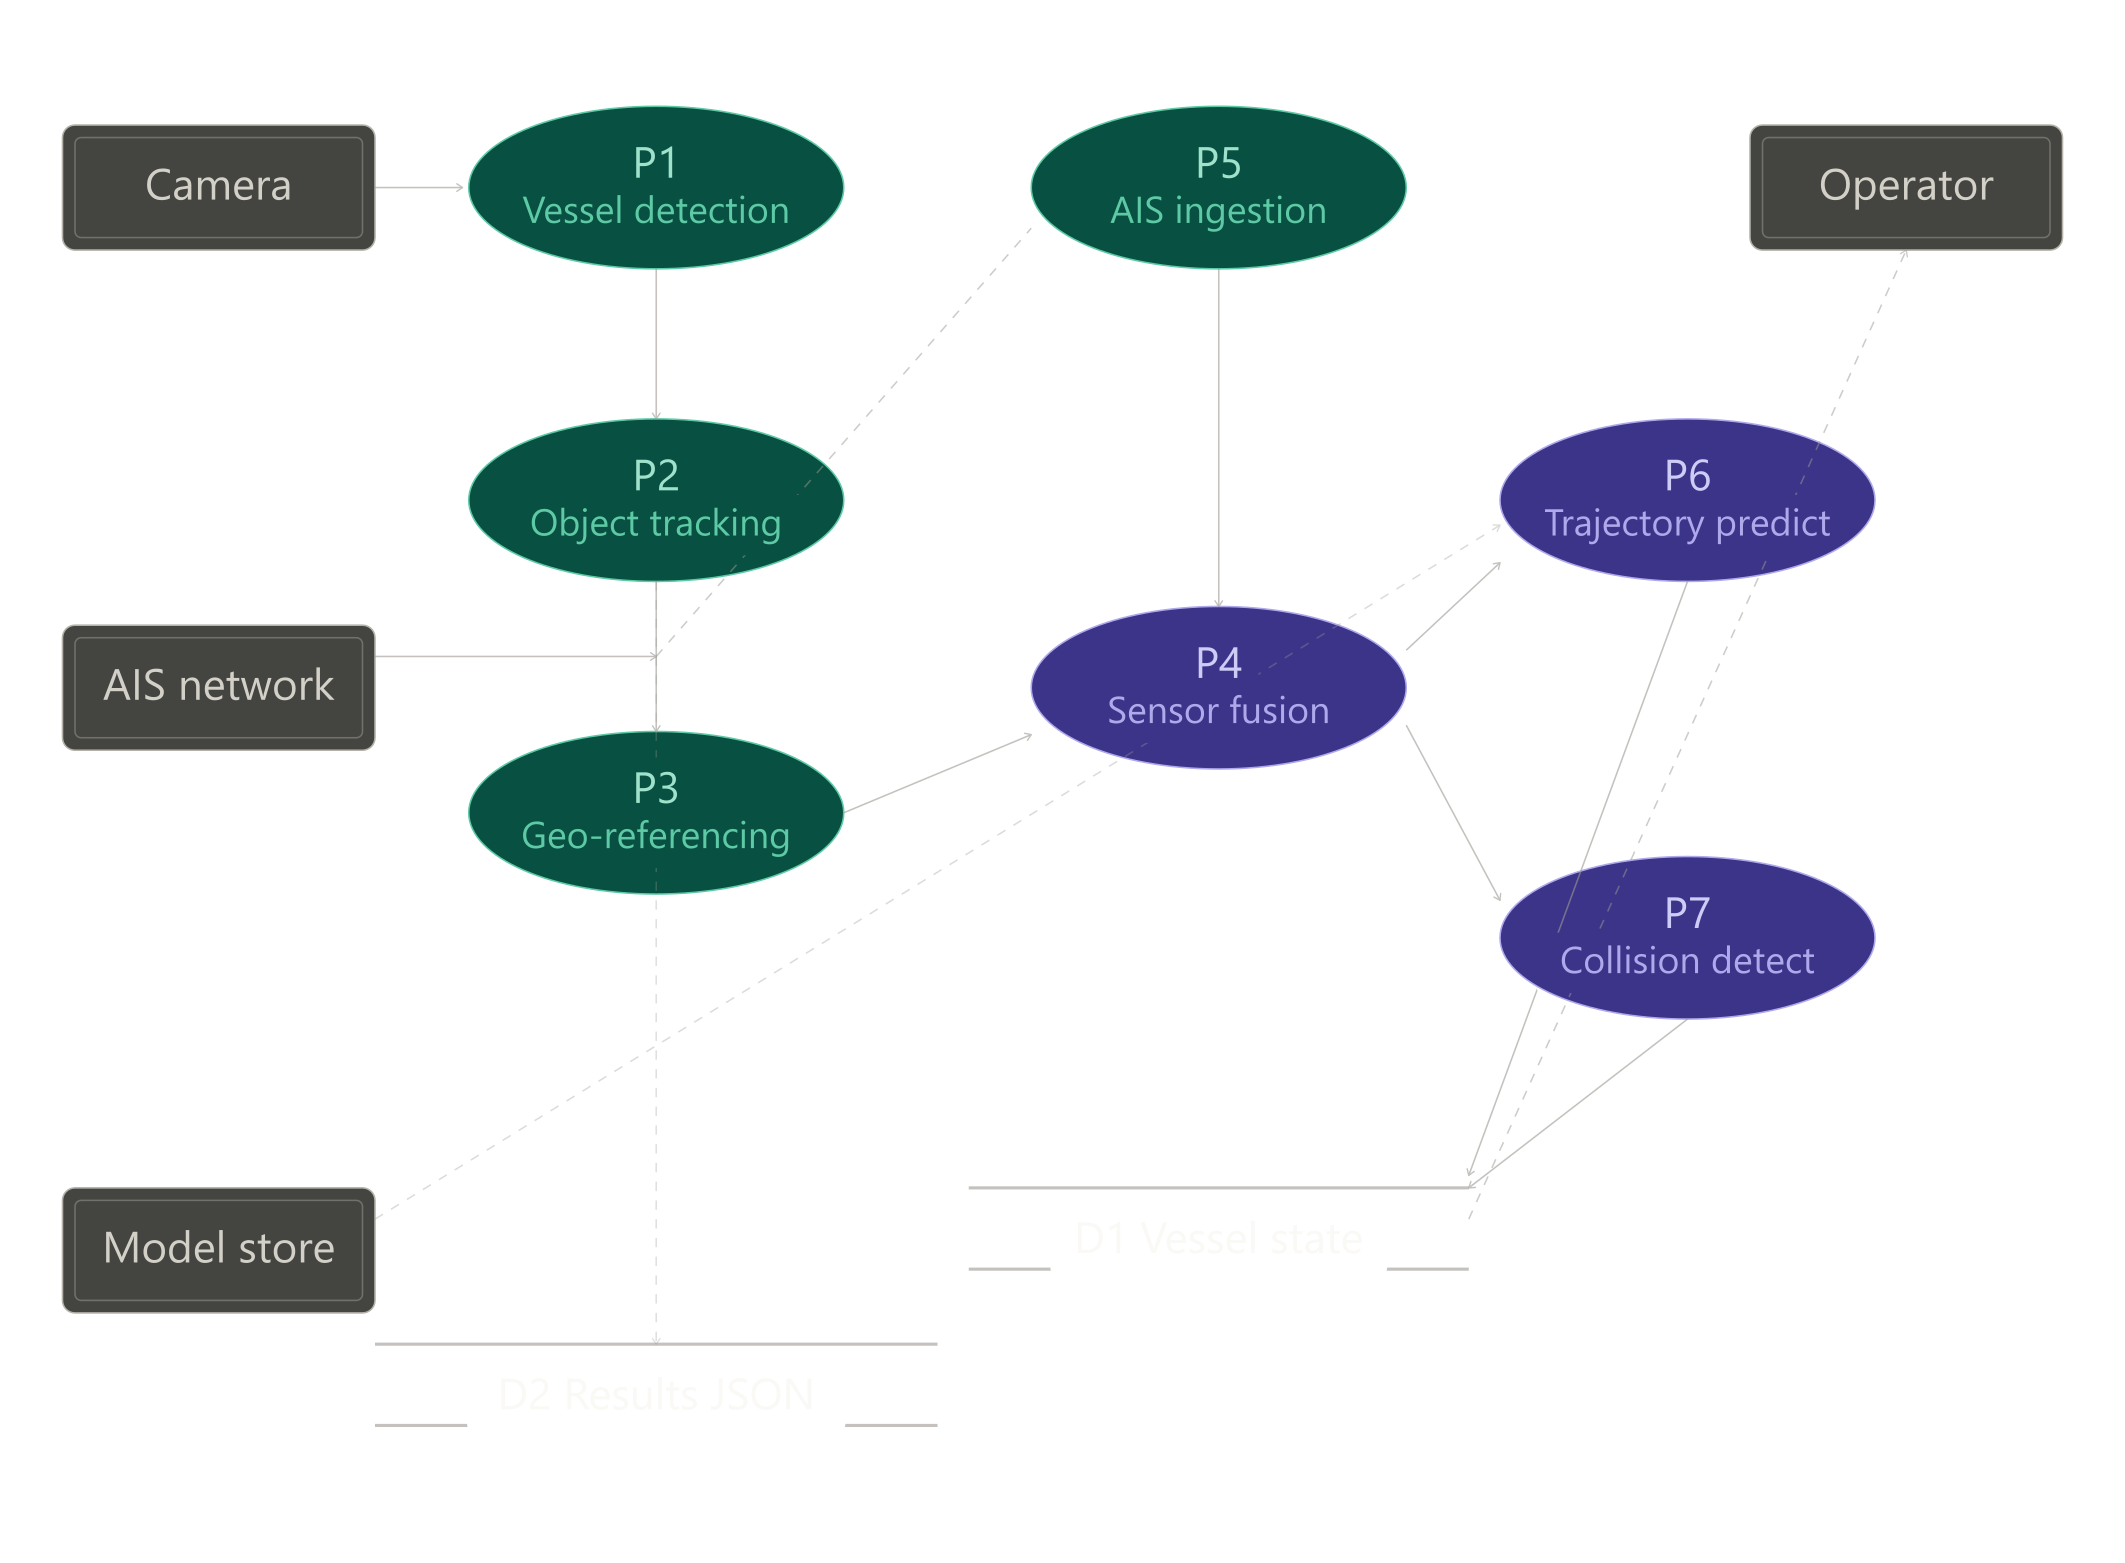
\includegraphics[width=0.95\textwidth]{Chapter3/Figures/dfd_level1_context.png}
\caption{Level-1 Data Flow Diagram of Proposed Maritime Surveillance System}
\label{fig:dfd1}
\end{figure}


\section{Module Description}

The proposed maritime surveillance system is composed of several interconnected modules that collectively enable real-time vessel monitoring, tracking, prediction, and visualization. Each module performs a dedicated task and contributes to the overall operation of the system.

\subsection{\texorpdfstring{\gls{ais}}{AIS} Data Acquisition Module}

The \gls{ais} data acquisition module is responsible for receiving and processing \gls{ais} telemetry data. The module extracts vessel identifiers, positional coordinates, speed information, and navigational parameters which are used for vessel association and monitoring.

\subsection{Video Processing Module}

The video processing module receives maritime video streams and performs frame extraction and preprocessing operations. Video frames are prepared for downstream computer vision operations.

\subsection{Vessel Detection Module}

The vessel detection module identifies ships within video frames using the \gls{yolov8} object detection model. The module generates bounding boxes around detected vessels and provides positional information for subsequent processing.

\subsection{Tracking Module}

The tracking module preserves vessel identities across consecutive frames and ensures continuity of observations. Tracking enables consistent monitoring of vessel movement throughout the surveillance period.

\subsection{Coordinate Transformation Module}

The coordinate transformation module converts image-space coordinates into geographic latitude--longitude coordinates. This conversion enables integration of visual detections with \gls{ais} telemetry data.

\subsection{Data Fusion Module}

The data fusion module combines information obtained from \gls{ais} telemetry and computer vision modules. The fusion process enriches vessel observations with navigational metadata and improves positional reliability.

\subsection{Trajectory Prediction Module}

The trajectory prediction module analyses historical movement patterns and predicts future vessel positions using a \gls{bilstm} network.

\subsection{Collision Detection Module}

The collision detection module analyses predicted trajectories and identifies possible collision scenarios among vessels operating within the monitored maritime region.

\subsection{Visualization Module}

The visualization module displays surveillance information, prediction outputs, and alert notifications through dashboard interfaces for operator monitoring and decision support.

\section{Summary}

This chapter presented a detailed account of the design and methodology 
underlying the proposed maritime surveillance system. The operational 
parameters of each module were established with explicit justification: the 
\gls{yolov8} detector was assigned a confidence threshold of 0.4 and an \gls{iou} 
threshold of 0.3 for \gls{nms}; the \gls{deepocsort} tracker was 
configured with a 90-frame history buffer, a minimum confirmation count of 3 
hits, a maximum track age of 30 frames, and a cosine similarity threshold of 
0.5 for \gls{reid}-based appearance matching; the \gls{fov} geo-referencing 
transform was anchored to the Singapore Strait camera position; the \gls{cv}-to-\gls{ais} 
fusion layer applied the Haversine nearest-neighbour method with a matching 
radius of 5.5\,km and a stale-record timeout of 300 seconds; and the \gls{seqtwo} 
\gls{lstm} predictor employed a bidirectional encoder with soft attention and a 
20-step autoregressive decoder, with kinematic linear regression as the 
fallback for tracks with fewer than 10 observations.

The pre-analysis stage evaluated candidate components across the full pipeline. 
Three object detection architectures --- Faster R-\gls{cnn}, \gls{ssdalg}, and the \gls{yolo} 
family (v5, v7, v8) --- were assessed under maritime-specific conditions 
including horizon glare, strong scale variation, and the requirement for 
real-time throughput. \gls{yolov8} was selected on the basis of its anchor-free 
regression head, enhanced feature pyramid neck, and superior small-object 
detection performance. For tracking, \gls{deepocsort} was preferred over 
motion-only trackers such as \gls{sort} and \gls{bytetrack} because its joint 
Kalman-filter--\gls{reid} association substantially reduced identity-switch events 
in occluded and crossing scenarios. For trajectory prediction, three 
candidate methods --- pure Kalman filter extrapolation, \glspl{gru}, and \gls{seqtwo} 
\glspl{lstm} --- were compared; the \gls{lstm} was chosen for its ability to model 
non-linear temporal dependencies and to focus selectively on the most 
informative history frames through its attention mechanism.

A rigorous mathematical foundation was established for each processing stage. 
The geo-referencing transform was formalised as an \gls{fov}-based linear 
approximation mapping pixel offsets from the frame centre to geographic 
latitude--longitude offsets (Equations~\ref{eq:lat_offset}--\ref{eq:gps_conversion}). 
The \gls{cv}-to-\gls{ais} spatial matching criterion was expressed using the Haversine 
great-circle distance formula 
(Equation~\ref{eq:haversine}). The \gls{lstm} architecture was formalised through 
the bidirectional encoder state update, the soft-attention weight computation, 
and the autoregressive decoder output equation 
(Equations~\ref{eq:LSTM1}--\ref{eq:LSTM2}). Together these formulations 
provide a complete theoretical account of the coordinate transformations, 
association decisions, and predictive inference steps that constitute the 
pipeline.

The two-phase pipeline architecture was then described in full, tracing the 
flow of data from raw video ingestion and live \gls{ais} stream reception through 
vessel detection, identity-preserving tracking, geo-referencing, 
nearest-neighbour \gls{ais} fusion, feature sequence construction, \gls{lstm} trajectory 
prediction, land-mask post-processing, and final output generation to the 
dashboard and results store.